\section{Modellazione dei requisiti del sistema}
Partendo da quanto detto fin ora è giunto il momento di modellare i requisiti del sistema.\newline

\noindent Al fine di ottenere una resa quanto più possibile chiara e completa si è scelto di \emph{modellare il sistema NeuroFrame da cinque differenti punti di vista}; in particolare, nel tentativo di rendere la fruizione il più semplificata possibile, \emph{i modelli verranno presentati partendo da aspetti maggiormente globali fino a raggiungere comportamenti del sistema più dettagliati}.\newline

\noindent I modelli scelti sono i seguenti:\newline
\begin{itemize}
  \item \emph{Casi d'uso}\\
  {Come naturale conseguenza della \emph{sezione 2.1} saranno formalizzati i casi d'uso del sistema.}
  \item \emph{Sottosistemi coinvolti}\\
  {Il macrosistema NeuroFrame è a sua volta composto da sottosistemi indipendenti che comunicano tra loro; qui dunque saranno presentati tali sottosistemi.}
  \item \emph{Flusso informativo}\\
  {Compreso quali siano i sottosistemi che compongono NeuroFrame verrà dunque esplicato il flusso informativo che intercorre tra di essi.}
  \item \emph{Analisi orientata agli oggetti}\\
  {Qui saranno esplicate ad alto livello le entità che caratterizzano il problema.}
  \item \emph{Analisi orientata agli stati}\\
  {Infine verranno esplicati i modelli di più difficile comprensione, rappresentanti gli stati che i sottosistemi possono assumere.}
\end{itemize}
\vspace{70mm}
\subsection{Casi d'uso}
Cominciamo modellando i casi d'uso del sistema nella sua interezza (\emph{figura 2.1}).
\begin{figure}[H]
  \centering
  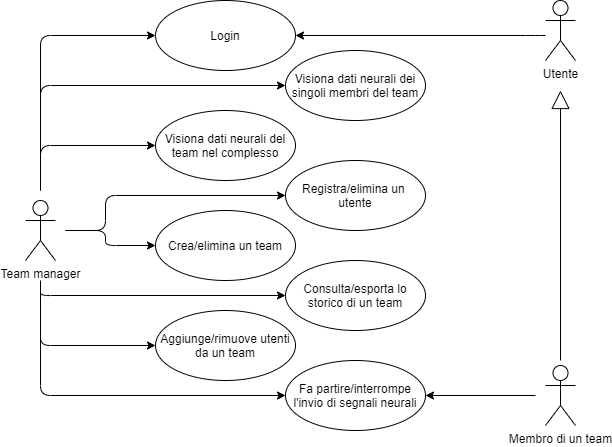
\includegraphics[width=0.7\textwidth]{img/casi_uso.png}
  \caption{Casi d'uso del sistema NeuroFrame}
\end{figure}
\noindent Troviamo due attori base: il {\bf Team manager} e l'{\bf Utente}; quest'ultimo, previa azione del Team manager, può specializzarsi nel {\bf Membro di un Team}.\newline
Analogamente il Membro di un Team può tornare ad essere un Utente base grazie all'intervento del Team manager.\newline

\noindent La possibilità di far iniziare e di interrompere lo streaming dei segnali neurali, così come il Login, è un caso d'uso comune a tutti gli attori.\newline

\noindent Le restanti casistiche sono interamente competenza del Team manager e possiamo distinguerle in due categorie:
\begin{itemize}
  \item \emph{Gestionali}\\
  {Egli si occuperà di creare/eliminare Utenti, aggiungere/rimuovere Utenti da un Team e crea/elimina i Team stessi.}
  \item \emph{Dati}\\
  {Potrà visionale il benessere cognitivo dei singoli individui così come il benessere del Team nel complesso; tali dati potranno anche essere esportati.}
\end{itemize}
\subsection{Sottosistemi coinvolti}
Vediamo ora i sottosistemi che compongono il macrosistema NeuroFrame (\emph{figura 2.2}).\newline
\begin{figure}[H]
  \centering
  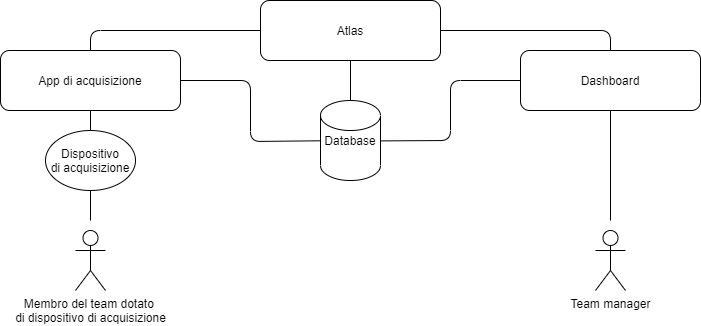
\includegraphics[width=0.9\textwidth]{img/NeuroFrameBase.png}
  \caption{Sottosistemi che compongono il macrosistema NeuroFrame}
\end{figure}

\noindent La {\bf piattaforma Atlas} (introdotta nella \emph{sezione 1.3}), si presenta come lo snodo centrale del macrosistema; essa riceve dati sullo stato cognitivo di un individuo e, dopo averli elaborati attraverso l'algoritmo che dà il nome all'intero progetto, li memorizza in un {\bf database}.\newline

\noindent Il compito di inviare i dati riguardo lo stato cognitivo viene svolto dall'{\bf App di acquisizione}. Ogni {\bf membro di un team} utilizza un'istanza di tale applicativo e, attraverso un {\bf Dispositivo di acquisizione}, ottiene passivamente un campionamento sul suo stato cognitivo. L'App di acquisizione inoltre comunica con il database al fine di autenticare un individuo attraverso le sue credenziali.\newline

\noindent Infine la {\bf Dashboard} si occupa di mostrare i dati elaborati dalla piattaforma Atlas ad un {\bf Team manager}; egli monitorerà le condizioni di un team ed avrà accesso a tutte le opzioni che gli permetteranno di gestire il team. La Dashboard comunica con il Database al fine di recuperare i dati elaborati (oltre che per autenticare i Team manager). La comunicazione con la piattaforma invece esiste al fine di poter verificare lo stato attuale di un membro del team (es: online o offline).\newline

\noindent Come si può notare dalla \emph{figura 2.2}, i due endpoint utilizzati dal cliente (App di acquisizione e Dashboard) non sono in comunicazione diretta tra loro, ma utilizzano Atlas ed il Database come intermediari.
\subsection{Flusso informativo}
Partendo dall'ultima osservazione, è opportuno dividere il flusso informativo in due diversi diagrammi così da facilitarne la comprensione.\newline

\noindent Il {\bf primo diagramma} (\emph{figura 2.3}) coinvolge il lato sinistro della \emph{figura 2.2}, ponendo il focus sull'{\bf App di acquisizione}.
\vspace{10mm}
\begin{figure}[H]
  \centering
  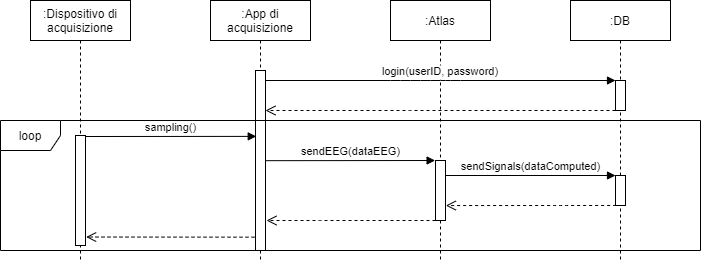
\includegraphics[width=1.0\textwidth]{img/diagramma_sequenza_alto_app_acquisizione.png}
  \caption{Diagramma di sequenza rappresentante il flusso informativo principale - lato applicativo di acquisizione}
\end{figure}
\vspace{5mm}
\noindent L'app di acquisizione effettua interrogazioni sul Database al fine di autenticare il membro del team.\newline

\noindent Il processo che porta ad ottenere un dato neurale elaborato comincia invece dal Dispositivo di acquisizione che, periodicamente, campiona lo stato del membro del team ed invia tale informazione all'App di acquisizione; essa a sua volta trasmette tale dato alla piattaforma Atlas, che si occuperà di estrapolare metriche rilevanti da tale dato.\newline
Al fine di rendere reperibili le metriche ottenute come ultimo passaggio Atlas salverà i risultati sul Database.\newline

\noindent Tale azione di campionamento verrà ripetuta a cadenza periodica.

\vspace{50mm}
\noindent Il {\bf secondo diagramma} (\emph{figura 2.4}) coinvolge invece il lato destro dell'analisi dei sottosistemi coinvolti (\emph{sezione 2.2.2}), chiarendo il flusso informativo che coinvolge la {\bf Dashboard}.
\vspace{10mm}
\begin{figure}[H]
  \centering
  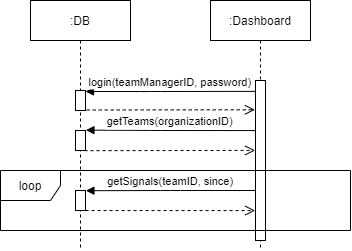
\includegraphics[width=0.55\textwidth]{img/diagramma_sequenza_alto_dashboard.png}
  \caption{Diagramma di sequenza rappresentante il flusso informativo principale - lato Dashboard}
\end{figure}
\vspace{5mm}
\noindent Ottenute le credenziali del Team manager, la Dashboard interroga il Database al fine di identificarlo; nel caso ciò vada a buon fine la Dashboard esegue una nuova interrogazione al fine di ottenere tutti i team esistenti nell'organizzazione.\newline

\noindent Una volta che il Team manager ha effettuato la scelta riguardo quale team monitorare, comincerà un'interrogazione periodica del Database da parte della Dashboard al fine di ottenere, se presenti, i nuovi dati elaborati appartenenti ad ogni membro del team.\newline

\noindent La richiesta di nuovi segnali viene eseguita dalla Dashboard a cadenza periodica.
\vspace{50mm}
\subsection{Analisi orientata agli oggetti}
Osservando il sistema dalla prospettiva di un'analisi degli oggetti ad alto livello possiamo visionare le entità nel diagramma in \emph{figura 2.5}.
\vspace{5mm}
\begin{figure}[H]
  \centering
  \includegraphics[width=0.9\textwidth]{img/Analisi orientata agli oggetti - NeuroFrame.png}
  \caption{Analisi orientata agli oggetti del sistema NeuroFrame}
\end{figure}
\vspace{5mm}
\noindent All'interno del sistema {\bf NeuroFrame} troviamo più {\bf Organizzazioni}, distinte dal loro identificativo.\newline

\noindent Per ogni Organizzazione abbiamo dei {\bf Team} e delle {\bf Persone}, che si specializzano in due diverse tipologie: {\bf Team manager} e membro del team ({chiamato per semplicità {\bf Utente}}); Persone e Team, così come le Organizzazioni, dispongono di un identificativo univoco.\newline

\noindent Ogni Utente può appartenere ad un solo Team per volta; il numero di Utenti appartenenti ad un Team ed il numero stesso di Team che possono esistere all'interno di un'Organizzazione è vincolato al \emph{tipo di licenza acquistata} da quest'ultima.\newline

\noindent Un Utente che appartiene ad un Team può cominciare un'{\bf Acquisizione}.\newline
Ogni Acquisizione è composta da uno o più segnali (contenti le metriche calcolate da Atlas ed il timestamp corrispondente all'istante temporale in cui è avvenuto il campionamento) ed utilizza necessariamente un solo {\bf Dispositivo di acquisizione} (che è posseduto da un'organizzazione).
\subsection{Analisi orientata agli stati}
Arriviamo dunque all'ultima analisi ed anche la più complessa.\newline
Qui è stato deciso di modellare indipendentemente gli stati di App di acquisizione e Dashboard, a seguito del requisito di indipendenza funzionale tra i due sistemi (definito nella \emph{sezione 2.1.2}).\newline

\noindent Per facilitare la lettura sono state colorate in verde le strade che conducono al flusso d'esecuzione corretto e di rosso, viceversa, a quello scorretto; inoltre le azioni periodiche sono state evidenziate in blu.\newline

\noindent Esplichiamo prima il comportamento dell'{\bf App di acquisizione} (\emph{figura 2.6}).
\vspace{5mm}
\begin{figure}[H]
  \centering
  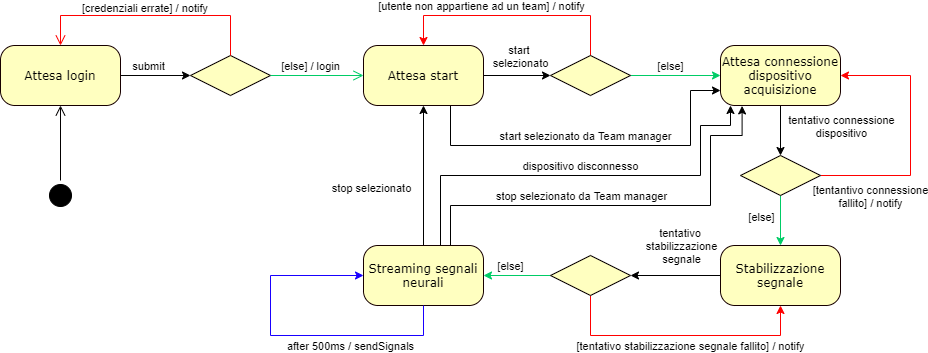
\includegraphics[width=1.0\textwidth]{img/App acquisizione - fsm.png}
  \caption{Analisi orientata agli stati - lato Applicativo d'acquisizione}
\end{figure}
\vspace{5mm}
\noindent Una volta effettuato il login il sistema attende l'input dell'Utente per procedere; un vincolo per transitare verso lo stato successivo però è rappresentato dall'appartenenza o meno ad un Team (come modellato nell'analisi orientata agli oggetti).\newline
Alternativamente è possibile transitare verso il prossimo stato attraverso input remoto del Team manager.

\noindent Si passa dunque prima ad una connessione al Dispositivo di acquisizione poi, previa connessione eseguita, ad una stabilizzazione del segnale.\newline

\noindent Una volta giunti allo stato in cui il sistema è correttamente in opera, l'app invia periodicamente (ogni 500 ms, al momento) alla piattaforma Atlas i dati ricevuti dal dispositivo di acquisizione in quel lasso temporale.\newline

\noindent Dallo stato di streaming dei segnali neurali si può uscire per tre ragioni: 
\begin{itemize}
  \item L'Utente interrompe volontariamente lo streaming
  \item Il Dispositivo di acquisizione si disconnette
  \item Via remoto il Team manager interrompe lo streaming dell'Utente
\end{itemize}

\vspace{5mm}
\noindent Modelliamo ora gli stati dell'applicativo {\bf Dashboard} (\emph{figura 2.7}).
\vspace{5mm}
\begin{figure}[H]
  \centering
  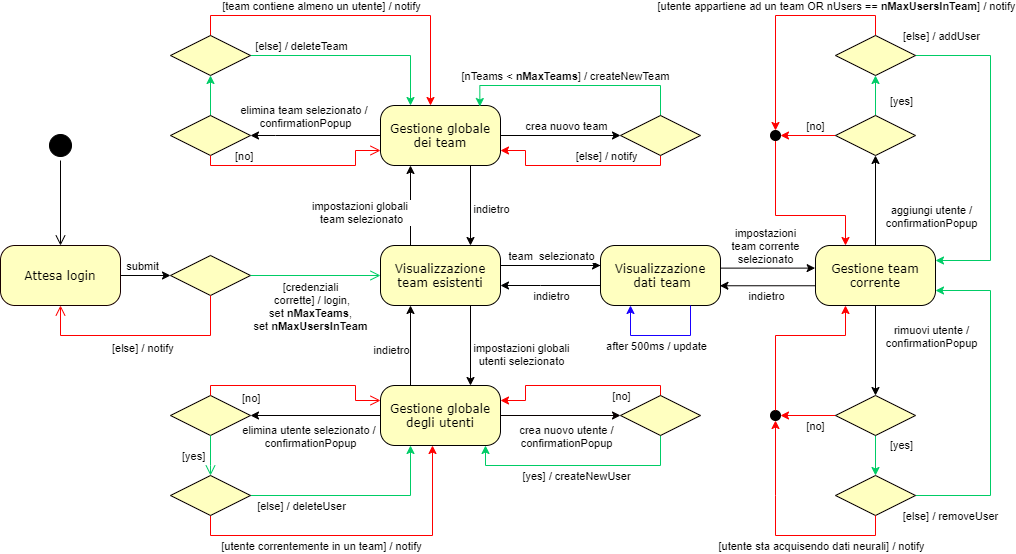
\includegraphics[width=1.0\textwidth]{img/Dashboard - fsm.png}
  \caption{Analisi orientata agli stati - lato Dashboard}
\end{figure}
\noindent Una volta effettuato il login, il Team manager visualizza i team esistenti all'interno dell'organizzazione.\newline
Da qui è possibile intraprendere tre strade. Due riguardano puramente aspetti gestionali:\newline
\begin{itemize}
  \item \emph{Gestione globale dei Team}\\
  {Qui il Team manager può creare nuovi Team (senza superare il limite imposto dalla licenza), oppure eliminare dei Team già esistenti.\newline
  Prima di eliminare un Team è necessario rimuovere tutti i suoi componenti al fine di evitare inconsistenze nel comportamento dell'App di acquisizione.}
  \item \emph{Gestione globale degli Utenti}\\
  {Qui invece è possibile creare nuovi utenti (il numero di Utenti esistenti non è limitato, a differenza del numero di componenti di un Team), o eliminare Utenti già esistenti.\newline
  Per eliminare un Utente è prima necessario rimuoverlo da un eventuale Team a cui partecipa, per le stesse motivazioni espresse nel punto precedente.}
\end{itemize}

\noindent La terza e ultima strada rappresenta il core dell'applicativo Dashboard: la visualizzazione dei dati neurali del Team.\newline
Qui, a cadenza periodica di 500 ms, il sistema interroga il Database richiedendo i nuovi dati disponibili relativi ai componenti del Team selezionato.\newline

\noindent Se prima vi era una gestione globale da questo stato è possibile transitare ad una gestione inerente solo al Team selezionato.\newline
Sarà possibile aggiungere Utenti (che già non appartengano ad un altro Team) ai componenti del Team selezionato (sempre non superando i limiti imposti dalla licenza acquistata) oppure rimuoverli (solo nel caso non stiano correntemente trasmettendo dati).
